\section{Reaching your full Potential}

\begin{quotex}
Every Real Man has realized all the possibilities of the human condition, but each one has done so in a way which is typical of him alone, and which differentiates him from all other Real Men. If that were not the case, how could there be room, in our world, even for beings who have not achieved that level? \flright{\textsc{Rene Guenon} \textit{in letter to Evola}}

\end{quotex}

\begin{wrapfigure}{rt}{0.4\textwidth}
\centering
 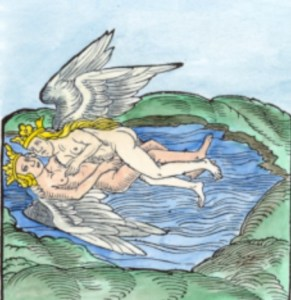
\includegraphics[scale=.4]{a20210321ReachingyourfullPotential-img001.jpg} 
\end{wrapfigure}

The first stage in esoteric teaching, the “Lesser Mysteries”, comprises everything related to the development of the possibilities of the human state. These possibilities transcend the activities of our ordinary life. The roles we play, such as family, occupation, and so on, are the fields of activity in which further development is made possible. Developing whatever talents we might have through education — the arts, science, sports, watching TV, and so on— may constitute the field of action that prepares us for higher possibilities, some obviously, better than others.

A fortiori, the search for powers or secret knowledge is fruitless, if not disadvantageous, from the esoteric perspective. These include:

\begin{itemize}
\item Fascination with vast conspiracy theories 
\item The search for psychic powers of all types 
\item The desire for mystical experiences 
\item Obsession with manifesting material objects 
\item Channeling higher beings 
\item Seeking secret knowledge of some sort 
\item Relying on psychedelics for spiritual experiences 
\end{itemize}
The common element is the focus on the corporeal and/or psychic worlds rather than the strictly spiritual part of oneself. \textbf{Rene Guenon} provides this admonition:

\begin{quotex}
[Psychic powers] are in fact a distraction in the rigorously etymological sense of the word. The one who lets himself be absorbed by the many activities of the corporeal world will never center his consciousness on higher realities, nor consequently develop within himself the corresponding possibilities. This will be all the more true for one who goes astray and disperses himself in the incomparably more vast and varied multiplicity of the psychic world, with its indefinite modalities. \flright{The “Rejection of Powers”, \emph{Perspectives on Initiation}}

\end{quotex}
This is not to deny the possibilities of such manifestations, which may arise as side-effects of mystical evolution. Nevertheless, our higher possibilities are not tied to any specific talents or abilities, since they are the principles which make those actions possible. From higher to lower, these are:

\begin{itemize}
\item True Will 
\item Consciousness 
\item Real I 
\end{itemize}
The attainment of these faculties completes the evolution of the possibilities of the human state, lifting the being to the Primordial State. Boris Mouravieff summarizes this succinctly:

\begin{quotex}
It is by this evolution that animal man can overcome Adam's Fall, can become a spiritual man, and so be initiated into divine wisdom. 

\end{quotex}
Then he is prepared for the Greater Mysteries.

\paragraph{Obstacles}
\begin{quotex}
Many are called but few are chosen. \flright{\textsc{Matthew 22:14}}

\end{quotex}
Here we encounter some immediate obstacles that prevent or discourage seekers.

\subparagraph{Unnecessary}
People believe that already have those faculties of a True Will, Consciousness, and a Real I. Hence, they don't see the need for esoteric training. They become more interested in phenomena.

\subparagraph{Explicit knowledge}
This type fails to understand the distinction between explicit and tacit knowledge. Explicit knowledge can be communicated through the written or spoken word. Tacit knowledge, on the other hand, cannot be communicated in that way. It is more like “knowing how” rather than in knowing. Tacit knowledge comes only by doing.

Like riding a bike or learning to swim, one has to actually do it. Reading a book about biking or swimming won't do it for you. Tacti knowledge is more effective if there is a guide, but most people are satisfied by reading or hearing theories about biking or swimming.

\subparagraph{Hard work}
\begin{quotex}
We can buy food for others; we can cook a dish with this food; we can serve it once it is cooked; we can cut it up; we can even act as if to put the food inside the mouth, as we do for a child or sick person. But at this point, each of us must make the necessary effort to swallow the food for ourselves; this cannot be done by anyone else. \flright{\emph{Gnosis I}}

\end{quotex}
Few people have the stamina or discipline to perform the exercises that transform explicit knowledge to tacit knowledge.

\subsubsection{Self-knowledge}
\begin{quotex}
When we close our eyes in an attempt to meditate, we are amazed to discover a boiler factory inside of us. \flright{\textsc{Joel Goldsmith}, \emph{The Art of Meditation}}

\end{quotex}
Meditation is sold today as an absolute good, that will relax us, lower blood pressure, and so on. However, if done properly, many, who believe that their inner life is nothing but Sunshine and Lollipops, are shocked to witness the “boiler factory” of irrelevant, fearful, or anxious thoughts that cast doubt rather than certainty.

It takes effort and persistence to get past that point.

\subparagraph{Inequality}
This teaching is the hardest to accept:

\begin{quotex}
Among several persons who receive an identical teaching, each one understands and assimilates it more or less completely and profoundly according to the range of his own intellectual possibilities, and in this way selection, without which there could be no genuine hierarchy, comes about quite naturally. \flright{\textsc{Rene Guenon}, \emph{Man and his Becoming according to the Vedanta}}

\end{quotex}
\paragraph{Higher Centers}
As mentioned in \textit{The Descent of the Absolute}\footnote{\url{https://www.gornahoor.net/?p=14019}}, the Emotional Center (animal soul) and Intellectual Center (intellectual soul) are divided into lower and higher centers. As we are born, the higher centers are undeveloped and are therefore only virtual. Esoteric training starts with the proper awakening or development of the higher centers.

Since our untrained emotional life is so erratic, mastery over the expression of the emotions is imperative in order to make further progress.

The Higher Emotional Center is located in the Heart, the seat of our Real I, the Sun center of our being. The Higher Intellectual Center is located at the level of the Head, the seat of consciousness.

\paragraph{Objective Art}
The first step in the in the development of the higher emotional center is to mitigate the effects of negative emotions. That opens up some space for more subtle emotions to manifest. Aids in the process include objective art, myths, and symbols. The focus of personal art is on the personality of the artist, while objective art is the reflection of higher ideas. The following passage refers to why, according to Plotinus, a sculpture is more beautiful than the block of stone from which it was carved.

\begin{quotex}
The real question is, why is the sculpted stone more beautiful? “The matter did not have this form, but it was in the one who thought, and before it came to the stone; but it was in the craftsman, not insofar as he had eyes or hands, but in that he shared in art” (Enneads V.8.1.16–19). If the sculpted stone is more beautiful than the lump, this is because thought, or idea, is more evident in it. The distinctive beauty of the sculpture, as opposed to the lump, is the form that it has received through the artist's work, which is an image of the form existing as pure thought-content, or idea, in the artist's mind. Consequently, the form, that is, the beauty, that renders the sculpture pleasing to behold is first and more truly in the artist's mind, as the paradigm of which the sculpture's beauty is an image. \flright{\textsc{Eric Perl}, \emph{Thinking Being}}

\end{quotex}
\paragraph{Myths and Symbols}
The purpose of Myths and Symbols is to reach these higher centers, the higher emotional and higher intellectual centers respectively. The attempt to understand myths and symbols by the lower mind will result in misinterpretation.

\paragraph{Sexual Sublimation}
Sexual energy can be redirected to the higher centers, which is the means to produce results.

\begin{quotex}
This consecration is produced by the sublimation of sex. Thus the circle closes itself. Each manifestation of life starts by a sexual act; at the end of the cycle, the activity of the sexual centre is manifested once more, but on a higher level, that of the higher centres, the level to which — by its nature — this centre belongs. \flright{\textit{Gnosis I}}

\end{quotex}
Ultimately, individual and group work will be replaced with Hieros gamos or polar couples. Since each one of the pair has a different way of knowing, their shared experiences enhance each other.

\begin{quotex}
The means … is to work as a couple. We must believe that in the new era which approaches, this method will be favoured more and more, will be protected, and will eventually become obligatory. However, for this esoteric work to be completed successfully by two people, it is essential that the two beings — man and woman — are integrally polar. 
\end{quotex}
\flrightit{Posted on 2021-03-21 by Cologero }

\begin{center}* * *\end{center}

\begin{footnotesize}\begin{sffamily}



\texttt{Greg on 2021-03-22 at 10:59 said: }

As to exercises does the form of Meditation matter? Is the Jesus prayer or say centering prayer effective in attaining these states or are other forms of exercises needed?


\hfill

\texttt{Tannheuser on 2021-03-22 at 12:47 said: }

I was actually just discussing this question of Objective vs. Personal art last night. 

I used the term “arbitrary” to describe what you call Personal art – to me it is boring because it does not participate in any universal idea or higher reality. That kind of art is usually a waste of time, because it doesn't offer any valuable possibilities to the one participating in it – just “A influences” imposing themselves and insisting on their own importance.

Interestingly, in contemporary art and entertainment, this arbitrary personal quality is the strongest in the so-called “high” arts (modern opera, painting, orchestral music, sculpture, architecture, and so on). Low or popular art often expresses less personal, more universal ideas, in the same way that folklore can preserve an echo the original spirit of a civilization long after the high art has become degenerate. Recently, however, there is a concerted effort to replace everything traditional even in low art with political propaganda (extending as far as 60 year old children's picture-books).


\hfill

\texttt{Arthur Konrad on 2021-03-23 at 09:20 said: }

@ Tannheuser,

Ever since the 19th century, opera and orchestral music is mostly an elaborate cacophony, operating on the same principle as a kid's toy made to produce some fabulous sound, after which the kid in question mutters `oooohhhh!' in awe – in other words, it is infantile. This is why Nietzsche loved Wagner, he had an infantile mentality. Most 19th century music was tailored to the tastes of women and effeminate men. Some operas of the romantic era are downright embarrassing. The bottom one and a half octave on the piano serves pretty much the same function. Most `virtuoso' pianists today play in a cacophonous way and abuse the bottom octaves as a rhythm section, and they think that a correct tempo does not exist. If you have healthy ears, you might as well shun piano performances for good, that thing is never going to get better.

Compare that nonsense to the masterpieces that are Baroque operas.


\hfill

\texttt{Paulo Adolpho on 2021-03-24 at 22:50 said: }

“A fortiori, the search for powers or secret knowledge is fruitless, if not disadvantageous, from the esoteric perspective. These include:

Fascination with vast conspiracy theories”

Cologero, why studying conspiracy theory, would it be negative? Don't you see that we must become aware, of who is trying to control and destroy this world, the anti-traditional forces?


\end{sffamily}\end{footnotesize}
